\section*{Exemplos}

\todo[inline]{Remover a secção ``Exemplos'', quando já não for necessária.}

\begin{info}
  São ilustradas de seguida algumas partes do documento.
  
  Esta secção não aparece no documento final!
\end{info}

\subsection*{Equações}

\begin{info}
Este texto é apenas um exemplo que precede uma equação.
\end{info}  

Equações simples podem ser inseridas em linha com o texto: 
a reta é \(y=mx+b\).

Equações mais complicadas devem ser separadas em linhas individuais e
numeradas sequencialmente à direita dentro de parêntesis.
Esta é a equação 2º grau genérica:

\begin{equation} \label{eq:1}
  ax^2+bx+cx=0
\end{equation}

Onde $a$ é o coeficiente de 2º grau; $b$ o de 1º grau; $c$ o
coeficiente independente da variável $x$, a determinar.

As equações devem ser referidas mantendo o seu número.
Por exemplo, a Equação~\ref{eq:2} resolve problemas formulados tal como 
mostrado na Equação~\ref{eq:1}.

\begin{equation} \label{eq:2}
  x=\frac{-b\pm \sqrt{b^2-4ac}}{2a}
\end{equation}

\lipsum[1]

\subsection*{Figuras e tabelas}

Todas as figuras e tabelas devem ser obrigatoriamente legendadas e
numeradas sequencialmente:

\begin{itemize}
\item as figuras devem ser legendadas por baixo;
\item as tabelas devem ser legendadas no topo. 
\end{itemize}

Mantenha as figuras centradas e em linha com o texto para que a
legenda apareça sempre colada com a imagem.

\begin{info}
As figuras devem flutuar livremente na página e ser referidas e
descritas no texto, com as fontes devidamente explicitadas, para
evitar o plágio\footnote{É importante não usar a opção 
destrutiva "[H]" para deixar o LaTeX fazer bem o trabalho de 
formação, tal como um tipógrafo faria!}.
\end{info}

Como exemplo, a Figura~\ref{fig:campus} %(retirada de\url{www.fe.up.pt}) 
mostra o \emph{campus} da FEUP. 
\lipsum[2]

\begin{figure}
\centering
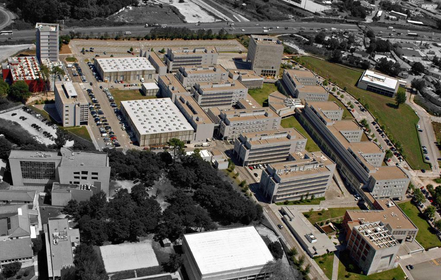
\includegraphics[width=0.7\textwidth]{campus}
\caption{Fotografia aérea do Campus da FEUP~\parencite{kn:figura}.} \label{fig:campus}
\end{figure}

%\lipsum[2]

%\begin{info}
%Pode ser reservado espaço para colocar, no futuro, uma figura; por
%exemplo, a Figura~\ref{fig:natal}.
%\end{info}
%
%\lipsum[3]
%
%\begin{figure} [b]
%  \centering
%  \missingfigure{Inserir a figura do Natal.}
%  \caption{O Natal no Campus da FEUP.} \label{fig:natal}
%\end{figure}

\lipsum[3]

\begin{info}
As tabelas devem flutuar livremente na página e ser referidas e
descritas no texto, com as fontes devidamente explicitadas, para
evitar o plágio.
\end{info}

A Tabela~\ref{tab:feup} % (excerto adaptado de ``A FEUP em números'', 2011)
serve para exemplificar como mostrar alguns valores que, neste caso, têm
a ver com alguns dados numéricos associados a recursos e investimentos
da FEUP no ano de 2011. 

\lipsum[4]

\begin{table}
  \centering
\caption[Physical Resources of \acs*{FEUP}]{Physical Resources of \acs*{FEUP}~\parencite{kn:feup}.}
\begin{tabular}{| l | S[table-number-alignment = right] |}
  \hline
  \textbf{Description} & \textbf{Quantity} \\ \hline
  \hline
  Total area of the FEUP campus & \SI{93918}{\square\meter} \\ \hline
  Green spaces & \SI{23}{\kilo\square\meter} \\ \hline
  Number of computers dedicated to teaching & \num{1815} \\ \hline
  Investment in laboratory equipment & \SI{1.46}{\mega\eurocurrency} \\ \hline
  Investment in Sustainability & \SI{31.4}{\kilo\eurocurrency} \\
  \hline
\end{tabular}
  \label{tab:feup}
\end{table}

%\lipsum[6]

\subsection*{Citações}

À medida que escreve o texto do relatório, deve indicar os trabalhos
de outros autores em que se baseia, sob a forma de citações.
Isto consiste em indicar de forma abreviada as fontes usadas às quais
foi buscar informação adicional para desenvolver o tema do seu
relatório.

Existem duas formas principais de citar:
\begin{itemize}
\item por \textbf{paráfrase}: interpretação do conteúdo original por
  palavras diferentes das da fonte consultada, indicando a fonte logo
  a seguir; ou 
\item 
  por \textbf{transcrição}: uso de um excerto do conteúdo original
  apresentando-o entre aspas, indicando a fonte logo a seguir.
\end{itemize}

As citações devem obedecer a um estilo normalizado.
De entre os muitos que existem, a Biblioteca da FEUP aconselha o
estilo Chicago (formato autor-data).

\begin{info}
De seguida exemplificam-se, ao acaso, algumas citações (por paráfrase)
de acordo com esse estilo.
\end{info}

A decisão de escolha de um tema para um trabalho académico pode
variar~\parencite{kn:Bel02-book}.
O tema pode ser pensado e escolhido pelo próprio estudante, ou a
partir de uma lista de temas já concebidos, com potencial interesse
para estudo~\parencite{kn:GLPR14-joPhysics}.

A cada citação ao longo do texto deve corresponder uma referência
indicada na lista final de referências
bibliográficas~\parencite{kn:Lip08,kn:MSS+12-wemep,kn:VKL+18-dtu}. 

É importante não esquecer que também as figuras (imagens, tabelas,
gráficos, etc.) provenientes de obras de outros autores (por exemplo 
obtidas através da Internet) devem ser citadas sempre, após as
respetivas legendas~\parencite{kn:GLPC22-torque}.

Para saber mais sobre este assunto e ver exemplos, consulte o guia
``Evitar o plágio: boas práticas no uso da informação'' disponível 
em \url{https://feup.libguides.com/plagio/citar}.  

Ainda mais um exmplo de citação com duas referências~\parencite{iso_19156_2011,ornelas2016} 
\lipsum[5]

\subsection*{Sistema Internacional de Unidades} \label{sec:siu}

\begin{info}
Exemplo da escrita de unidades e valores de acordo com as normas do Sistema Internacional de Medidas.
\end{info}

Deve ser usado o pacote \texttt{siunitx}\footnote{Manual disponível em 
\url{https://ctan.org/pkg/siunitx}.} para escrever valores, unidades, etc., 
de acordo com as regras do Sistema Internacional de Unidades 
(ver \url{https://physics.nist.gov/cuu/Units/checklist.html}). 

Por exemplo:
\SI{50}{\kilo\gram}, 
\SI{15}{\celsius}, 
\SI{20,01}{\meter\per\second}, 
\SI{120}{\kilo\byte\per\second}, 
\SI{34}{\percent}, 
\SI{289300.00}{\eurocurrency}, 
\SI{28.3}{\mega\eurocurrency}, 
\num{10245.450234}.

A Tabela~\ref{tab:feup2} % (excerto adaptado de ``A FEUP em números'', 2011)
serve para exemplificar o alinhamento nas colunas com números, e nada tem a ver com qualquer dado numérico associado aos recursos e investimentos da \acs*{FEUP} em 2025.

\begin{table}
  \centering
  \caption[Physical Resources of \acs*{FEUP}]{Physical Resources of \acs*{FEUP}~\parencite{kn:feup}.}
  \begin{tabular}{@{}S@{}}
    \toprule
    {Some Values} \\
    \midrule
    2.3456 \\
    34.2345 \\
    -6.7835 \\
    90.473 \\
    5642.5 \\
    1.2e3 \\
    e4 \\
    \bottomrule
  \end{tabular}
  \label{tab:feup2}
\end{table}

\lipsum[6]

\subsection*{Acrónimos e abreviaturas} \label{sec:acronym}

\begin{info}
Exemplo do uso de acrónimos.  O pacote \LaTeX\ usado faz as formatações requeridas.
\end{info}

Da primria vez os acrónimos \ac{IA} e \ac{ML} são expandidos e, mais tarde, podemos simplesmente referir-nos a \ac{IA} ou a \ac{ML}.

Na tecnologia moderna, a \ac{PLN} desempenha um papel crucial nos assistentes virtuais e nos \emph{chatbots} e dependemos de hardware \ac{GPU} para modelos de aprendizagem profunda e de \acp{API} para aceder aos dados e, \ac{WWW}, podemos usar a codificação \ac{ASCII}.

\subsubsection{Use de Acrónimos em Títulos \acs*{FEUP}}

Os acrónimos também podem ser colocados no plural: \acp{GPU} são amplamente utilizados na computação de alto desempenho.
As formas possessivas também são suportadas: \ac{IA}'s impactam a sociedade de forma profunda.

\lipsum[7]

\subsection*{Código}

\begin{info}
De seguida é ilustrado como incluir código no documento.
\end{info}

Listing~\ref{code:useless} 
\lipsum[8]

\begin{lstlisting}[language=Python, caption=Python example, label=code:useless]
# Take the user's input
words = input("Enter the text to translate to pig latin: ")
print(f"You entered: {words}")

# Break apart the words into a list
words = words.split(' ')

# Use a list comprehension to translate words greater than or equal to 3 characters
translated_words = [(w[1:] + w[0] + "ay") for w in words if len(w) >= 3 ]

# Print each translated word
for word in translated_words:
    print(word)
\end{lstlisting}

\subsection*{Uso das macros}

\begin{info}
De seguida é ilustrada a utlização de macros \LaTeX{} definidas no
preâmbulo.
De salientar o uso da macro \verb!\class{}! para classes, métodos e componentes.
\end{info}

O \windspt, retirado do \windscannerpt, usa o \svg\ \ldots\ como em \class{Student.calculate-age()}.
\lipsum[9]

\lipsum[10]

\subsection*{O travessão}

Sobre o uso do hífen e do travessão\footnote{"Ciberdúvidas da Língua Portuguesa", \url{https://ciberduvidas.iscte-iul.pt/consultorio/perguntas/o-uso-do-hifen-e-do-travessao/31251}}: 
\begin{enumerate}
    \item O hífen (U+002D, Alt + 0045, ``-''): sem espaços em branco (-);
    \item O travessão (ou travessão duplo)/em-dash (U+2014, Alt + 0151): em português, envolto em espaços em branco (---);
    \item O traço de ligação/en dash (U+2013, Alt + 0150): sem espaços em branco (--);
    \item O sinal matemático de subtração (igual ao hífen): sem espaços em branco (–).
\end{enumerate}

\lipsum[11]

\subsection*{As aspas}

Sobre as aspas  em \LaTeX, ou é usado o glifo diretamente (U+201C e U+201D), ou então são feitas com o acento para trás no início e a plica no fim, como em ``exemplo''\footnote{What is the best way to use quotation mark glyphs? 
\url{https://tex.stackexchange.com/questions/531/what-is-the-best-way-to-use-quotation-mark-glyphs}}.

\begin{info}
As partes componentes subsequentes que constituem o corpo do texto
devem ser estruturadas em secções, estimando-se que até 3 níveis seja
o suficiente para este tipo de trabalho.

Para saber mais consulte o tutorial online 
``\href{https://docs.google.com/document/d/1TDC1behVq8x7fQL4CcPEEh_np5GXviJevQxnQ9gbiJs/edit}
{Guia de Apoio à Publicação}''.
Note-se que as seções aí indicadas podem ser adaptadas em função do tema
ou profundidade do estudo a desenvolver.
\end{info}

\begin{info}
Não é costume haver cabeçalhos de secções seguidas sem texto no meio.
A compreensão dos textos pode ser melhorada através de uma pequena 
introdução às secções seguintes colocada entre uma secção e a sua primeira sub-secção. Estes textos ligan a narrativa
do documento.
\end{info}
